\documentclass[border=5pt]{standalone}
\usepackage[utf8]{inputenc}
\usepackage{amsmath}
\usepackage{amssymb}

\usepackage{tikz}
\usetikzlibrary{shapes.geometric, arrows}
\usetikzlibrary{automata,positioning}

\tikzstyle{startstop} = [rectangle, rounded corners, minimum width=3cm, minimum height=1cm,text centered, draw=black, fill=red!30]
\tikzstyle{io} = [trapezium, trapezium left angle=70, trapezium right angle=110, minimum width=3cm, minimum height=1cm, text centered, draw=black, fill=blue!30]
\tikzstyle{process} = [rectangle, minimum width=3cm, minimum height=1cm, text centered, draw=black, fill=orange!30]
\tikzstyle{decision} = [diamond, minimum width=3cm, minimum height=1cm, text centered, draw=black, fill=green!30]
\tikzstyle{arrow} = [thick,->,>=stealth, rounded corners]
\tikzstyle{fdot} = [circle, minimum width=4pt, fill]
\tikzstyle{line} = [thick,>=stealth, rounded corners]

\begin{document}

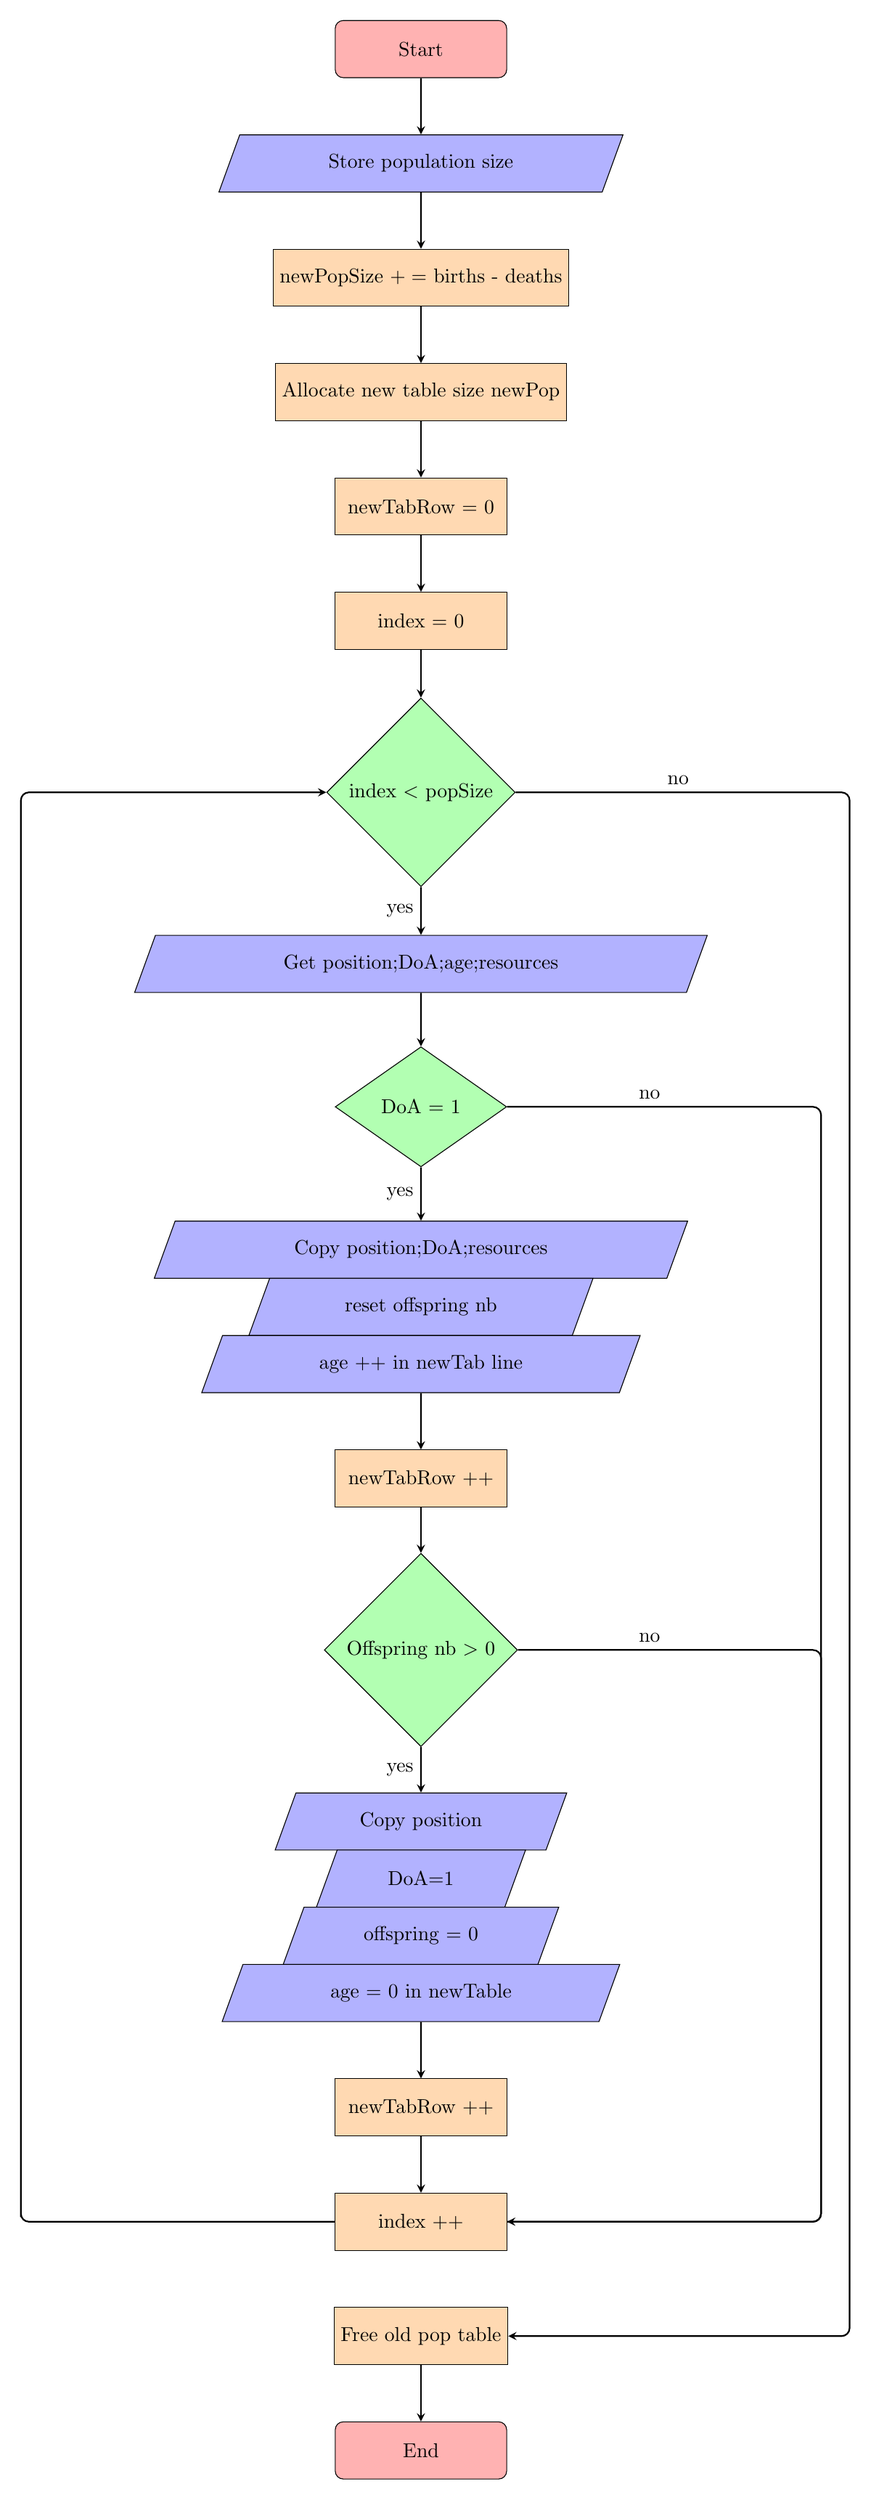
\begin{tikzpicture}[node distance=3cm]

\node (start) [startstop] {Start};
\node (out1) [io, below of=start, yshift=1cm] {Store population size};
\node (pro1) [process, below of=out1, yshift=1cm] {newPopSize $+=$ births - deaths};
\node (pro2) [process, below of=pro1, yshift=1cm] {Allocate new table size newPop};
\node (pro3) [process, below of=pro2, yshift=1cm] {newTabRow = 0};
\node (pro4) [process, below of=pro3, yshift=1cm] {index = 0};
\node (dec1) [decision, below of=pro4] {index $<$ popSize};
\node (in1) [io, below of=dec1] {Get position;DoA;age;resources};
\node (dec2) [decision, below of=in1, yshift=0.5cm] {DoA $=$ 1};
\node (out2) [io, below of=dec2, yshift=0.5cm] {Copy position;DoA;resources};
\node (out3) [io, below of=out2, yshift=2cm] {reset offspring nb};
\node (out4) [io, below of=out3, yshift=2cm] {age ++ in newTab line};
\node (pro5) [process, below of=out4, yshift=1cm] {newTabRow ++};
\node (dec3) [decision, below of=pro5, yshift=0cm] {Offspring nb $>$ 0};
\node (out5) [io, below of=dec3, yshift=0cm] {Copy position};
\node (out6) [io, below of=out5, yshift=2cm] {DoA=1};
\node (out7) [io, below of=out6, yshift=2cm] {offspring = 0};
\node (out8) [io, below of=out7, yshift=2cm] {age = 0 in newTable};
\node (pro6) [process, below of=out8, yshift=1cm] {newTabRow ++};
\node (pro7) [process, below of=pro6, yshift=1cm] {index ++};
\node (pro8) [process, below of=pro7, yshift=1cm] {Free old pop table};
\node (stop) [startstop, below of=pro8, yshift=1cm] {End};

\draw [arrow] (start) -- (out1);
\draw [arrow] (out1) -- (pro1);
\draw [arrow] (pro1) -- (pro2);
\draw [arrow] (pro2) -- (pro3);
\draw [arrow] (pro3) -- (pro4);
\draw [arrow] (pro4) -- (dec1);
\draw [arrow] (dec1) -- node[anchor=east] {yes} (in1);
\draw [arrow] (dec1) -| node[anchor=south, xshift=-3cm] {no} + (7.5,-0.5) |- (pro8);
\draw [arrow] (in1) -- (dec2);
\draw [arrow] (dec2) -- node[anchor=east] {yes} (out2);
\draw [line] (dec2) -| node[anchor=south, xshift=-3cm] {no} + (7,-0.5) |- (pro7);
\draw [arrow] (pro7) -| + (-7,0) |- (dec1);
%\draw [arrow] (out2) -- (out3);
%\draw [arrow] (out3) -- (out4);
\draw [arrow] (out4) -- (pro5);
\draw [arrow] (pro5) -- (dec3);
\draw [arrow] (dec3) -- node[anchor=east] {yes} (out5);
\draw [arrow] (dec3) -| node[anchor=south, xshift=-3cm] {no} + (7,-0.5) |- (pro7);
%\draw [arrow] (out5) -- (out6);
%\draw [arrow] (out6) -- (out7);
%\draw [arrow] (out7) -- (out8);
\draw [arrow] (out8) -- (pro6);
\draw [arrow] (pro6) -- (pro7);
\draw [arrow] (pro8) -- (stop);

\end{tikzpicture}

\end{document}